\chapter{Problemspezifikation}\label{problemspezifikation}

In diesem Kapitel wird die Selbsteinbettung von Taskgraphen in Mehrprozessorsystemen vorgestellt. Am Beispiel von einem Network-on-Chip (NoC) werden dessen Architektur und ihre Besonderheiten näher betrachtet. Das Constraint-Satisfaction-Problem (CSP) wird definiert und die Bedingungen (engl. \textit{Constraints}) für die Architektur festgelegt. Anschließend werden die theoretischen Grundlagen des Min-Conflicts-Embedders erläutert.

\section{Selbsteinbettung in Mehrprozessorsysteme}
In einem Mehrprozessorsystem \cite{Mehrprozessorsysteme} arbeiten mehrere Zentralprozessoren zusammen. 
Mehrprozessorsysteme erlauben die Verteilung der Aufträge auf mehrere physische Zentralprozessoren und helfen somit den Durchsatz zu erhöhen. Das Betriebssystem verteilt die Anwendungen (engl. \textit{Application}) und deren Teilaufgaben (engl. \textit{Task}) an die Zentralprozessoren.  \\ \ \\
Bei der betrachteten Architektur (Abbildung ~\ref{fig:nocbild}) handelt es sich um ein heterogenes Mehrprozessorsystem. Kennzeichnend dafür ist die Verwendung verschiedener Typen von Zentralprozessoren. Diese werden im Weiteren Kacheln genannt. Die einzelnen Kacheln sind in einem Netzwerk -- einem sogenannten Network-on-Chip (NoC) \cite{mappingNocArchitectures} \cite{NOC} -- miteinander verbunden. Das Netzwerk ist zu einem regelmäßigen rechteckigen Gitter von Kacheln geordnet, welches N hoch und M breit ist. Die direktbenachbarten Kacheln sind mit gerichteten Links  $l_i \in L$ (Abbildung ~\ref{fig:links}) in beide Richtungen verbunden. Die Kacheln k $\in$ K sind durch die Koordinaten (x,y) definiert:
\begin{equation} 
 \forall k \in K: k = \{(x, y) | 0 \leq x < N , 0 \leq y < M \}
\label{kacheln}
\end{equation}

Eine Kachel kann einen Task ausführen, wenn alle Constraints erfüllt sind. Einer dieser Randbedingungen ist der Max-Hop-Constraint. Diese besagt, dass zwei miteinander agierende Tasks eine Manhattan-Distanz  $d_m$ (Formel \ref{formel2}) nicht überschreiten dürfen. 

\begin{equation}
d_m (k_1,k_2) = \mid k_1.x - k_2.x \mid + \mid k_1.y - k_2.y \mid 
\label{formel2}
\end{equation}

\begin{figure}[H]\centering
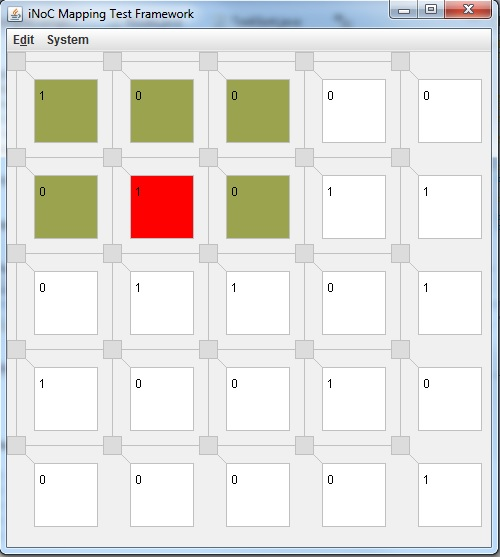
\includegraphics[width = 70mm]{bilder/NoC.jpg}
\caption{Simulation eines heterogenes Network-On-Chip: Die belegten Kacheln sind mit grün und die defekten Kacheln mit rot markiert. In jeder Kachel steht der Ressourcentyp (im Beispiel 0 oder 1).}\label{fig:nocbild}
\end{figure}

\begin{figure}[H]\centering
  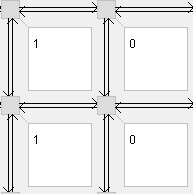
\includegraphics[width = 30mm]{bilder/Links.jpg}
  \caption{Die benachbarten Kacheln sind mit gerichteten Links in beide Richtungen verbunden.}\label{fig:links}
\end{figure}
\ \\
Jede Anwendung, die aus mehreren Teilaufgaben, den sogenannten Tasks, besteht, besitzt einen Taskgraphen (Abbildung ~\ref{fig:taskgraph}). Dieser wird zur Entwurfszeit des Programms angefertigt und stellt die Anforderungen, die für eine erfolgreiche Einbettung notwendig sind, graphisch dar.


\begin{figure}[H]\centering
  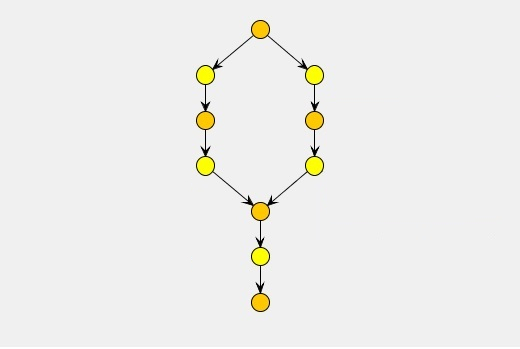
\includegraphics[width = 150mm]{bilder/taskgraph2.jpg}
  \caption{Der Taskgraph besteht aus orangefarbenen Task- und gelbgefärbten Kommunikationsknoten}\label{fig:taskgraph}
\end{figure}
\ \\
Eine Applikation besteht aus miteinander verbundenen Taskknoten $t \in T$ und Kommunikationsknoten $c \in C$. Es sind nur Kanten zwischen diesen beiden Knotentypen erlaubt. Außerdem besitzt jeder Kommunikationsknoten \textbf{genau} eine Eingangskante und eine Ausgangskante. Dem Task- und dem Kommunikationsknoten werden verschiedenartige Bedingungen übergeben, die zu erfüllen sind. Die verschiedenen Typen von Constraints sind je nach Anwendungsgebiet erweiterbar.

\begin{itemize}
\item Taskknoten $t_i\in T$
\begin{itemize}
\item \textit{TypeConstraint}: \\
Der Task benötigt einen bestimmten Ressourcentyp.
\item \textit{TaskWorkloadConstraint}: \\
Der Task nimmt die  Kachel zu einem gewissen Prozentsatz in Anspruch.
\item \dots 
\label{Taskknoten}
\end{itemize}
\item Kommunikationsknoten $c_i \in C$:
\begin{itemize}
\item \textit{BandwidthConstraint}: \\
Jede Kommunikation benötigt jeden Link auf der Route eine bestimmte Bandbreite.
%\item $c_i$.messageSize: Die Nachrichtengröße
%\item $c_i$.period: Das Intervall, in dem die Nachrichten geschickt werden /todo{Abstand in dem die Nachrichten geschickt werden?}
\item \textit{MaxHopConstraint}: \\
Die Route der Kommunikation darf nicht länger als eine maximale Manhattan-Distanz sein.
\item \dots
\label{Kommunikationsknoten}
\end{itemize}

\label{Randbedingungen}

\end{itemize}

\ \\
Das Ziel des Algorithmus ist es, für jeden Task eine Kachel zu finden, so dass alle Anforderungen des Taskgraphen erfüllt sind. Ist dies nicht möglich, soll der Algorithmus sich beenden und einen Fehlschlag der Einbettung melden. Im Abschnitt \ref{minConflicts} (Implementierung in Abschnitt \ref{minConflictImpl}) wird mit dem Min-Conflicts-Embedder ein heuristischer  Ansatz vorgestellt. Es gibt auch die Möglichkeit, die Problemstellung mit dem systematischen Ansatz zu lösen. Dies wird in der Quelle \cite{jaeger} näher erläutert.


\section{Constraint--Satisfaction--Problem (CSP)}

Das Problem der Taskeinbettung lässt sich als Constraint-Satisfaction-Problem (CSP) formulieren. Ein CSP wird mit dem Tripel $(V, D, B)$ (Definition \ref{Def:CSP})  beschrieben. Ziel des Constraint-Satisfaction-Problems ist es, eine global konsistente Wertebelegung für alle Constraint-Variablen zu finden. Das bedeutet, es müssen alle Bedingungen erfüllt sein. Eine Bedingung ist genau dann erfüllt, wenn die Wertezuweisungen den Anforderungen der Bedingung entspricht \cite{handbuchkuenstlicheIntelligenz}. Die Bedingungen lassen sich wie in \cite{jaeger}  umformulieren. \\
\\


\begin{def1}[Constraint-Satisfaction-Problem \cite{artificialIntelligence}] \label{Def:CSP}
\begin{itemize}
\item V = \{$V_1$, $V_2$, \ldots , $V_n$\} ist eine endliche Menge von Variablen.
\item D = \{$D_1$, $D_2$, \ldots , $D_n$\} sind die Wertebereiche von V mit den Werten $d_i \in D_i$.
\item B = \{$B_1$, $B_2$, \ldots , $B_m$\} ist die Menge der Bedingungen, wobei jedes Randbedingung $B_j(V_j)$ eine Teilmenge $V_j = \{V_{j_1},\ldots,V_{j_m}\} \subseteq V$ der Variablen zueinander in Verbindung setzt und deren gültige Wertekombinationen auf eine Teilmenge von $D_{j_1} \times \cdots \times D_{j_m}$ beschränkt.
\end{itemize}
\end{def1}

\section{Min-Conflicts-Embedder}\label{minConflicts}
Die Min--Conflicts--Heuristik ist in der Praxis eine häufig eingesetzte Methode zum Lösen von CSPs. Es handelt sich nicht um ein systematisches Verfahren wie beim Backtracking, sondern um ein Heuristisches. Als Startpunkt wird eine zufällige Belegung der Variablen erzeugt. Falls dies keine Lösung des CSPs ist, wovon auszugehen ist, wird eine kon\-flikt\-er\-zeu\-gen\-de Variable zufällig ausgewählt. Dieser wird ein Wert zugewiesen, der möglichst wenige Randbedingungen verletzt.\\ \\
Wie bei anderen stochastischen Methoden besteht auch hier die Gefahr, dass das System in einem lokalen Minimum terminiert. Das bedeutet, dass keine weiteren Verbesserungen
erzielt werden können, eine Lösung für das CSP aber noch nicht gefunden
wurde. Falls dies der Fall ist, muss eine erneute zufällige Belegung der Variablen erzeugt werden und eine neue Runde beginnt. Eine Tabu-Liste kann dabei helfen, Belegungen, die zu einem lokalen Minimum geführt haben, nicht mehr zu wählen. Nach einer vorher festgelegten Anzahl von Runden beendet sich die Heuristik und das Scheitern der Einplanung wird ausgegeben. So kann es vorkommen, dass die Min--Conflicts-Heuristik keine konsistente Lösung findet, obwohl eine im Constraint--System vorhanden ist.\\ \\
Oftmals wird die Heuristik verwendet, wenn sich das Constraint--System geringfügig verändert hat und für das vorherige System schon eine Lösung vorhanden ist. Aus diesem Grund wird der Algorithmus auch als "heuristisches Reparieren" \cite{cspsolvingRepairMethod} bezeichnet.\\ \\
